\section{Research Design}\label{sec:design}

In a given social media platform, we collect data from a user base $\mathcal{U}$. For a given period of time, we observe the digital traces of the focal user $u\in \mathcal{U}$ from $N$ social media posts, denoted by $p_1^u, p_2^u, \ldots, p_N^u$, ordered in time $\tau_1^u < \tau_2^u < \ldots < \tau_N^u$. Our objectives are two-folded: (1) We aim to detect all the \entity, denoted by $e_1^u, e_2^u, \ldots, e_M^u$, from a user's historical observations $\boldsymbol{H}^u = \left[\left(p_1^u, \tau_1^u\right), \left(p_2^u, \tau_2^u\right), \ldots, \left(p_N^u, \tau_N^u\right)\right]$. Here, the number of \entity, $M$, does not necessarily equal the number of social media posts $N$. One can extract zero, one or many \entity from a single social media post. (2) We aim to predict the probability of a user labeled as depression\footnote{we identify a depression user $u$ who has explicitly mentioned that they have been diagnosed with depression}. For simplicity, we describe our method for a given user $u$ and drop the superscript $u$ hereafter. The same analysis is applied to all the other users $\mathcal{U} \setminus u$. 

To achieve these two goals, we propose the DeepKnowledge Framework for Depression Detection (referred to as \model hereafter) from digital traces on social media. \model consists of three modules. 
The first module extracts the predefined entities that are informative of depression based on the medical knowledge (Section~\ref{sec:design:module1}). The second module establishes the medical knowledge foundation for our prediction and provides the source of depression knowledge for the third module (Section~\ref{sec:design:module2}). The third module leverages the knowledge from the first two modules and develops a knowledge-driven attention-based sequence model for depression prediction (Section~\ref{sec:design:module3}). 
The specific model components in these modules are shown in the first column in Table~\ref{tbl:design:knowledge}. The design rationale, the related medical knowledge, and the research gaps addressed for each model component are articulated in the second and third columns in Table~\ref{tbl:design:knowledge}. Figure~\ref{fig:design:model} shows the architecture of the proposed \model. 

\begin{table}[h]
    \caption{Notation} \label{tb:Notation}
    \small
    \centering
    \begin{threeparttable}
    \begin{tabular}{L{0.1\textwidth} L{0.85\textwidth}}
    \toprule
    Notation &  \multicolumn{1}{c}{Description} \\ \midrule
    $P_j$ & $j$-th social media posts of an individual \\
    $N_i$ & $i$-th diagnosis-related named entities of an individual\\
    $X_i$ & the BERT embedding of $i$-th named entitities of an individual \\
    $\tau_i$ & the time at which the post where $i$-th named entities belong is published \\
    \bottomrule
    \end{tabular} 
    \end{threeparttable}
    \end{table}

\begin{figure}[h]
    \centering
    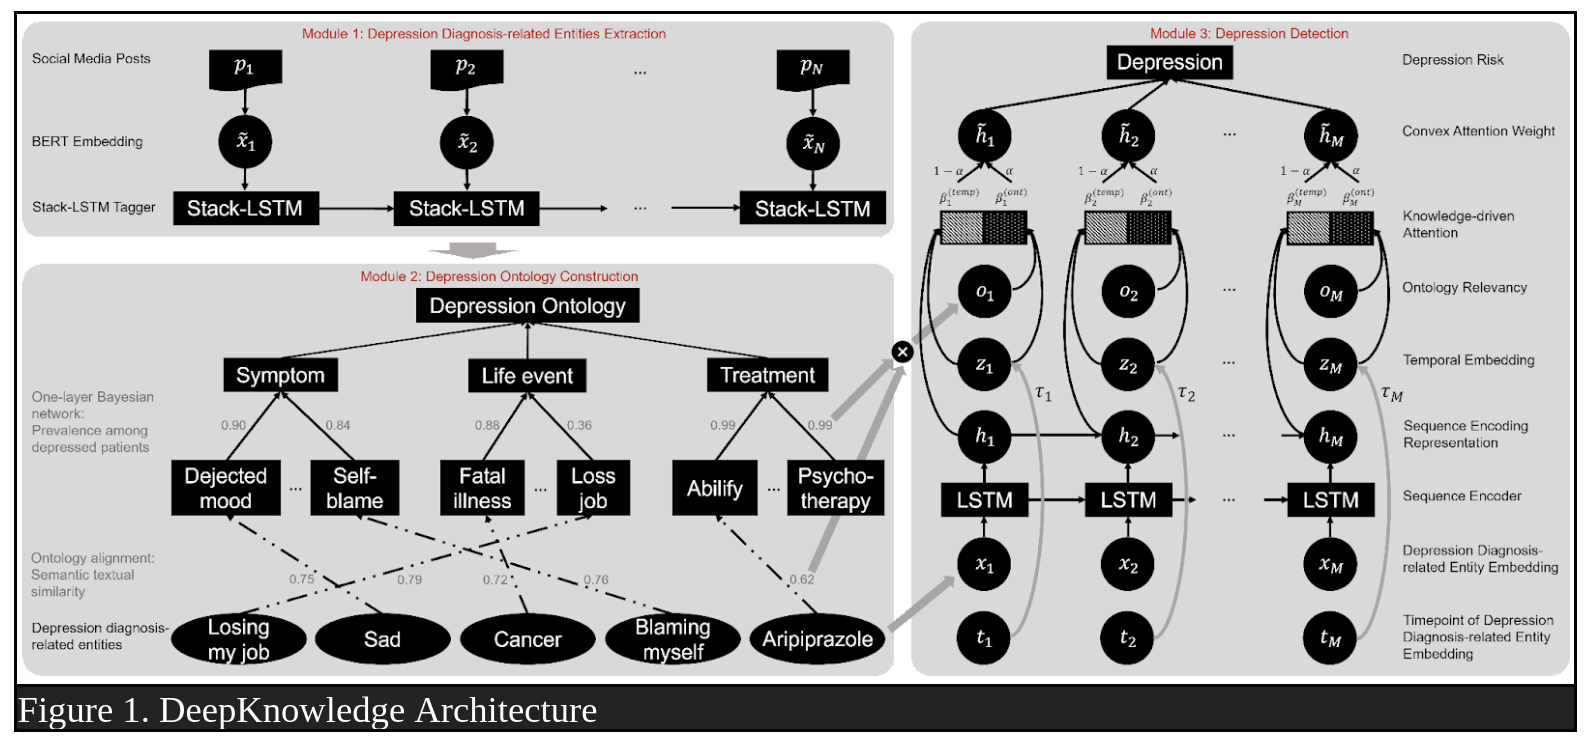
\includegraphics[width=1.0\textwidth]{imgs/method.png}
    \caption{The architecture of \model}
    \label{fig:design:model}
\end{figure}


\begin{algorithm}[!th]
%\small
% \footnotesize
\SetAlgoLined
    \textbf{Input:} Data $X=\{x_i\}_{i=1}^{N}$, labels $Y = \{y_i\}_{i=1}^{N}$ \\
    \textbf{Output:} $\Phi_{\Theta}$:targeted neural encoder for $X$, $U=\{u_c\}_{i=1}^{C}, V=\{v_c\}_{i=1}^{C}$: positive and negative anchors for each of $C$ classes\\
%\textbf{Output:} 
%%$Z_{A|B}$: conditional latent  representation for atoms,   %$Z_B$:latent representation for bonds, 
%$Z_M$:latent representation for atom $M$, 
%$\log P_\mathcal{M}(M)$: logarithmic  likelihood of molecule $M$. \\
%\KwResult{}
%\For{ \text{sampled mini-batch} $X=\{x_i\}_{i=1}^{N}$ }
\For{ each epoch }
{
    \mytag{Step 1:} Sampling mini-batch $X=\{x_i\}_{i=1}^{n}$ \\
    \mytag{Step 2:} Generating data representations $Z=\{z_i\}_{i=1}^{n} = \Phi(\{x_i\}_{i=1}^{n})$ \\
    \mytag{Step 3:} Computing  the supervised contrastive loss $\mathcal{L}_{\text{Supervised Contrastive} }  = \mathcal{L}_{\text{Contrastive Cross Entropy} }  + \lambda \mathcal{L}_{\text{Supervised Contrastive Regularizer}} $  by Eq.~\ref{eq:multi-cbce} or Eq.~\ref{eq:multi-csce} \\
    \mytag{Step 4:} Updating $\Theta, U, V$ by minimizing above loss. 
}
\quad \textbf{Return:} $\Phi_{\Theta}$, $U, V$\\
    \caption{ The learning framework of our \model \label{alg:scehr}}
\end{algorithm}

\begin{table}[h]
\centering
\caption{Design Guidelines for DeepKnowledge}~\label{tbl:design:knowledge}
\resizebox{\textwidth}{!}{
\begin{mytabular}[2]{L{2cm}L{2cm}m{8cm}m{5cm}}
    \toprule
    \multicolumn{2}{l}{Model Components} & Medical Knowledge & Research Gaps \\
    \midrule
    \multicolumn{2}{l}{\blap{Depression diagnosis-related \\ entities extraction}}
    & Depression diagnosis-related symptoms, life events, and treatments are critical indicators of depression and are essential for timely intervention~\citep{beck_depression_2014}.
    & Depression diagnosis-related symptoms, life events, and treatments are often overlooked in depression detection studies \\
    \multicolumn{2}{c}{\blap{Knowledge-driven depression\\ detection}}
    & Depression diagnosis-related symptoms, life events, and treatments are sequential data. Sequence encoders, such as LSTM, can model such time-series historical events~\citep{xie2022care}.
    & \multirow{7}{*}{\blap{Depression knowledge is \\ under-explored in machine \\ learning models for \\ depression detection.}} \\
    & Time & Time recency is essential knowledge to determine depression. More recent depression diagnosis-related symptoms, life events, and treatments have more salient influence than the older counterparts~\citep{heikkinen_recent_1994} & \\
    Depression knowledge & Ontology & Depression ontology information, including symptom, life event, and treatment, is indicative of depression risk~\citep{beck_depression_2014} & \\
    & Attention & Different depression diagnosis-related symptoms, life events, and treatments carry distinct influence on the depression risk. They can be weighted to provide an more accurate depression prediction~\citep{beck_depression_2014,xie_readmission_2021} & \\
    \bottomrule
\end{mytabular}
}
\end{table}



\subsection{Module 1: Depression Diagnosis-related Entities Extraction}\label{sec:design:module1}

Corresponding to the upper left block of Figure~\ref{fig:design:model}, we define \entity as personal encounters related to disease symptoms, major life events, and depression treatments. Figure~\ref{fig:design:extract} shows an example. To extract these entities from social media posts, we leverage a state-of-the-art transition-based NER model~\citep{lample_neural_2016}. This model has an architecture that chunks and labels a sequence of inputs using Stack-LSTM~\citep{dyer_transition-based_2015} which allows the NER model to work like a stack that maintains a “summary embedding” of its input. The text representation scheme of this model is BERT~\citep{devlin_bert_2018}. Let $\boldsymbol{P} = \left(p_1,p_2,\ldots, p_N\right)$ and $\boldsymbol{E} = \left(e_1,e_2,\ldots, e_M\right)$ be user's observed social media posts~\red{user generated contents sound better?} and extracted \entity respectively. The module learns a mapping: $\boldsymbol{P} \longrightarrow \boldsymbol{E}$. We also obtain the learnt language understanding representation for these \entity, $\boldsymbol{X} =\left(x_1,x_2,\ldots, x_M\right)$.  

\begin{figure}[h]
    \centering
    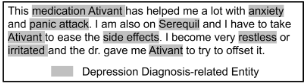
\includegraphics[width=0.4\textwidth]{imgs/example-ner.png}
    \caption{An example of \entity}
    \label{fig:design:extract}
\end{figure}

Unlike prior studies that use the entire social media post as the input, we leverage the detected \entity as our model input. These entities are more medically relevant and practically meaningful for explanation. Understanding what \entity are important in predicting depression is also critical for interventions. To name a few, if entities related to family emergencies are found to be salient predictors of the prediction, the social media platform can act on this information to offer online solutions for the emergencies and resources for support groups. If entities related to adverse drug events greatly contribute to the prediction, the platform can subsequently recommend guidelines from trusted health organizations (e.g., CDC, NIH, and WHO) on what actions to take to alleviate such adverse events. 


\subsection{Module 2: Depression Ontology Construction}\label{sec:design:module2}

The \entity extracted in module~\hyperref[sec:design:module1]{1} have uneven contributions to depression status~\red{uneven? equal contributions?}. Based on our depression ontology literature review, we construct a depression ontology as the medical knowledge base in our model. As shown in module~\hyperref[sec:design:module2]{2} of Figure~\ref{fig:design:model}, the medical terminologies used in the depression diagnosis can be divided into three subclasses~\citep{apa_diagnostic_2013,beck_depression_2014,almqvist_impact_2008}: Symptom, Life event, and Treatment. The Symptom class is a collection of depression symptoms. The Life event class is a collection of major life event changes that may cause or exacerbate depression. The Treatment class includes antidepressants and depression therapies.  The prevalence among depression patients is from the medical literature~\citep{beck_depression_2014}. The semantic textual similarity of each extracted \entity $e_i$ w.r.t the medical terminologies $mt_j$ corresponds to their dense representations inferred by the pre-trained language model $\phi$ (e.g., BERT~\citep{devlin_bert_2018}):

\begin{equation} \label{eq:cosine-similarity}
    \mathtt{sm}(e_i, mt_j) = \cos(\phi(e_i), \phi(mt_j))
\end{equation}

\subsection{Module 3: Time-Knowledge Fusion Depression Detection}\label{sec:design:module3}

Given a user's \entity sequence $\boldsymbol{X} = \left(e_1, e_2, \ldots, e_M\right)$ obtained from module~\hyperref[sec:design:module1]{1}, our goal is to predict the depression status of the focal user. The entity sequence encodes more relevant and practically more meaningful depression information than the original social media posts and creates a better user-level representation to identify depression. 

The right block of Figure~\ref{fig:design:model} shows the architecture of our proposed framework which can be break into three parts: 

The conventional LSTM model treats each depression diagnosis-related entity equally. Therefore, each entity would contribute equal information to the prediction. In reality, the importance of each entity based on the depression knowledge (i.e., relevancy to depression diagnosis and its time recency) is essential knowledge for this prediction. Based on this observation, DeepKnowledge embeds such depression knowledge into our sequence model. For each depression diagnosis-related entity $x_i$, we first learn an effective representation $h_i$ via an LSTM layer:

\begin{equation} \label{eq:lstm}
h_i = f^{(\mathtt{lstm})}\left(h_{i-1}, x_i\right)
\end{equation}